\subsection{Separability is Equivalent to Regular Colourability}

We start by showing that the "$\REC$-separability problem" is equivalent,
under polynomial time reductions, to the "regular colourability problem". To make our statement precise, we need some terminology.

\AP Let $\intro*\kREC$ be the class of languages expressed by unions of products of $k$ regular languages which form a partition, that is (in the binary case), relations of the form $(L_{i_1} \times L_{j_1}) \cup \dotsb \cup (L_{i_\ell} \times L_{j_\ell})$, with $i_1,j_1,\hdots,i_\ell, j_\ell \in \lBrack 1,k \rBrack$, for some regular partition\footnote{By ``regular partition'',
we mean that $L_1, \dotsc, L_{k}$ is a partition of $\Sigma^*$, and that moreover
each $L_i$ is a "regular language".} $L_1, \dotsc, L_{k}$ of $\Sigma^*$ and $\ell \in \N$.

Note that $\REC = \bigcup_k \kREC$.
For instance, $(aa)^* \times (aaa)^*$ belongs to $\kREC[4]$ but not to $\kREC[3]$
since, for any $k\in \N$, we have that $(aa)^* \times (aaa)^* \in \kREC[k]$ "iff"
there exists a regular partition of $a^*$ into $k$ languages "st" both
$(aa)^*$ and $(aaa)^*$ can be expressed as the union of some of these languages.\footnote{To get the
upper bound $k=4$, consider the partition $\tup{L_6, L_3, L_2, L_\bot}$ where $L_6 = (a^6)^*$,
$L_3 = (a^3)^* \smallsetminus L_6$, $L_2 = (a^2)^* \smallsetminus L_6$ and $L_\bot = a^* \smallsetminus (L_2 \cup L_3 \cup L_6)$.}

\AP Let us denote by $\intro*\Id$ the identity relation (on any implicit alphabet). Observe that $\Id$ is "automatic" but not "recognizable".

\begin{theorem}
    \AP\label{thm:reg-colourability-equiv-separability}
    There are polynomial-time reductions: 
    \begin{enumerate}
        \itemAP\label{item:reg-colourability-equiv-separability-1} from "$\REC$-separability@@problem" to "finite regular colourability@@problem", 
        \itemAP\label{item:reg-colourability-equiv-separability-2} from "finite regular colourability@@problem" to "$\REC$-separability@@problem", and
        \itemAP\label{item:reg-colourability-equiv-separability-3} from "$k$-regular colourability@@problem" to "$\kREC$-separability@@problem", for every $k > 0$.
    \end{enumerate}
    Further, the last two reductions are so that the second relation in the instance of the separability problem is the identity $\Id$.
\end{theorem}
   
\begin{proof}[Proof of \eqref{item:reg-colourability-equiv-separability-2} and
    \eqref{item:reg-colourability-equiv-separability-3}.]
    We start with the last two reductions.
    Given an "rational graph" $\AutGraph{V}{\+E}$ over an alphabet $\Sigma$, consider the instance
    $\tup{\+R_1, \+R_2}$ for the "$\REC$-separability problem", where 
    $\+R_1 = \+E$ and $\+R_2 = \Id$. 
    If $\AutGraph{V}{\+E}$ is "$k$-regular colourable" via the colouring $V_1, \dotsc, V_k$ then the $\kREC$ relation
    $\bigcup_{i \neq j} V_i \times V_j$ "separates@@rel" $\+R_1 = \+E$ and $\+R_2 = \Id$. 
    Conversely, if a $\kREC$ relation $\+R \subseteq \Sigma^* \times \Sigma^*$ on the regular 
    partition $V_1 \dcup \dotsb \dcup V_k = \Sigma^*$ "separates@@rel" $\+R_1$ and $\+R_2$, then $\bigcup_{i \neq j} V_i \times V_j$ also "separates@@rel" $\+R_1$ and $\+R_2$, and this implies that $V_1, \dotsc, V_k$ is a "$k$-colouring" for $\AutGraph{\Sigma^*}{\+E}$, and in particular
    for $\AutGraph{V}{\+E}$.
\end{proof}

\AP For the first reduction, let us introduce some terminology.
Given two relations $\+R_1$, $\+R_2$ over $\Sigma^*$, say that
$u \in \Sigma^*$ is ""compatible"" with
$u' \in \Sigma^*$ when for all words $v \in \Sigma^*$:
\begin{center}
    \intro*\compL: $\tup{u,v} \in \+R_1 \Rightarrow \tup{u',v} \not\in \+R_2$%
    ,\hphantom{\text{ \fancyand }}
    \intro*\compR: $\tup{v,u} \in \+R_1 \Rightarrow \tup{v,u'} \not\in \+R_2$,\\
    \intro*\compLpr: $\tup{u',v} \in \+R_1 \Rightarrow \tup{u,v} \not\in \+R_2$%
    \hphantom{,}\text{ \fancyand }
    \intro*\compRpr: $\tup{v,u'} \in \+R_1 \Rightarrow \tup{v,u} \not\in \+R_2$.
\end{center}
\AP
Define the ""incompatibility graph"" $\intro*\incompGraph{\+R_1}{\+R_2}$
as the graph whose vertices are all words of $\Sigma^*$,
and with an edge from $u$ to $v$ whenever $u$ is not "compatible" with $v$.
Note that $\incompGraph{\+R}{\Id}$ is exactly the graph $\AutGraph{\Sigma^*}{\+R}$.

\begin{example}%
    \AP\label{ex:equal-length-plusone}%
    Let $\Sigma = \{a,b\}$, $\+R_1$ be the equal-length relation,
    and
    \[
        \+R_2 = \{\tup{u, ua} \mid u \in \Sigma^*\} \cup \{\tup{u, ub} \mid u \in \Sigma^*\},
    \]
    which we depict in \Cref{fig:equal-length-plusone-relation}.
    Then, $u$ is "incompatible" with $u'$ if $|u| = |u'|+1$ (this is given by \compL~or \compR),
    or if $|u'| = |u|+1$ (this is given by \compLpr~or \compRpr).
    This gives rise to the "incompatibility graph" of
    \Cref{fig:equal-length-plusone-incompatibility}.
    \begin{marginfigure}[-8em]%
        \centering
        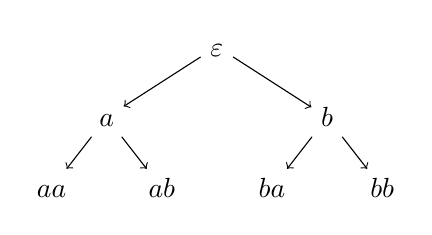
\begin{tikzpicture}
            \tikzset{
	level distance=.9cm,
	level 1/.style={sibling distance=2.8cm},
	level 2/.style={sibling distance=1.4cm},
	level 3/.style={sibling distance=.7cm},
	edge from parent/.style={draw,->}
}

\node (t) {$\varepsilon\vphantom{b}$}
	child {node {$a\vphantom{b}$}
		child {node {$aa\vphantom{b}$}
		}
		child {node {$ab$}
		}
	}
	child {node {$b$}
		child {node {$ba$}
		}
		child {node {$bb$}
		}
	};
        \end{tikzpicture}
        \caption{\AP\label{fig:equal-length-plusone-relation}%
            The relation $\+R_2$ of \Cref{ex:equal-length-plusone},
            restricted to words of length at most 2.
        }
    \end{marginfigure}%
    \begin{marginfigure}%
        \centering
        \begin{tikzpicture}
            \tikzset{
	level distance=.9cm,
	level 1/.style={sibling distance=2.8cm},
	level 2/.style={sibling distance=1.4cm},
	level 3/.style={sibling distance=.7cm},
	edge from parent/.style={}
}

% Coloring
\fill[rounded corners, fill=cBlue, opacity=.5]
	(-2.5,-2.05) rectangle (2.5,-1.57)
	(-.3,-0.25) rectangle (.3,0.23);
\fill[rounded corners, fill=cYellow, opacity=.5]
	(-1.65,-1.15) rectangle (1.65,-0.67);
% Tree
\node (eps) {$\varepsilon\vphantom{b}$}
	child {node (a) {$a\vphantom{b}$}
		child {node (aa) {$aa\vphantom{b}$}
		}
		child {node (ab) {$ab$}
		}
	}
	child {node (b) {$b$}
		child {node (ba) {$ba$}
		}
		child {node (bb) {$bb$}
		}
	};
\draw[<->] (eps) edge (a)
	(eps) edge (b)
	(a) edge (aa)
	(a) edge (ab)
	(a) edge (ba)
	(a) edge (bb)
	(b) edge (aa)
	(b) edge (ab)
	(b) edge (ba)
	(b) edge (bb);
        \end{tikzpicture}
        \caption{\AP\label{fig:equal-length-plusone-incompatibility}%
            "Incompatibility graph" $\incompGraph{\+R_1}{\+R_2}$ and its "2-regular colouring".%
        }
    \end{marginfigure}%

    Note that while neither $\+R_1$ nor $\+R_2$ are "recognizable",
    they are "separable@@rel" by the "recognizable" relation
    $\+S$ consisting of all pairs $\tup{u,v}$ such that $|u|$ and $|v|$ have the same parity.
    Moreover, $\incompGraph{\+R_1}{\+R_2}$ is "2-regular colourable", the two colours being
    the words of even and odd length.
\end{example}

\begin{proposition}
    \AP\label{prop:incomp-is-automatic}
    If $\+R_1$ and $\+R_2$ are "automatic", then so is $\incompGraph{\+R_1}{\+R_2}$.
    Moreover, we can build an automaton for $\incompGraph{\+R_1}{\+R_2}$ in polynomial time in the size of the automata for $\+R_1$ and $\+R_2$.
\end{proposition}

\begin{proof}
    By definition, the "incompatibility relation" $\incompGraph{\+R_1}{\+R_2}$ can be written as
    $\+R_{\neg\compL} \cup \+R_{\neg\compLpr} \cup \+R_{\neg\compR} \cup \+R_{\neg\compRpr}$, where:
    \begin{align*}
        \+R_{\neg\compL} &\defeq \big\{ \tup{u,u'} \in \Sigma^* \times \Sigma^* \;\big\vert\; \exists v \in \Sigma^*,\; \tup{u,v} \in \+R_1 \land \tup{u',v} \in \+R_2 \big\} \text{,}\\
        \+R_{\neg\compLpr} &\defeq \big\{ \tup{u,u'} \in \Sigma^* \times \Sigma^* \;\big\vert\; \exists v \in \Sigma^*,\; \tup{u',v} \in \+R_1 \land \tup{u,v} \in \+R_2 \big\} \text{,}\\
        \+R_{\neg\compR} &\defeq \big\{ \tup{u,u'} \in \Sigma^* \times \Sigma^* \;\big\vert\; \exists v \in \Sigma^*,\; \tup{v,u} \in \+R_1 \land \tup{v,u'} \in \+R_2 \big\} \text{, and}\\
        \+R_{\neg\compRpr} &\defeq \big\{ \tup{u,u'} \in \Sigma^* \times \Sigma^* \;\big\vert\; \exists v \in \Sigma^*,\; \tup{v,u'} \in \+R_1 \land \tup{v,u} \in \+R_2 \big\}
    \end{align*}
    Observe that starting from automata for $\+R_1$ and $\+R_2$, then for each
    of the relation $\+R_{\neg\compL}$, $\+R_{\neg\compLpr}$, $\+R_{\neg\compR}$ or $\+R_{\neg\compRpr}$, we can build an "automaton@@sync" recognizing them
    using a product construction, which can be implemented in polynomial time.\footnote{More precisely, in this product construction the states are $Q_1 \times Q_2$
    where $Q_i$ is the set of states of an "automaton@@sync" $\+A_i$ for $\+R_i$. Then,
    for each transition
    \[
        q_i \transition{\tup{a,b}} q'_i
    \]
    in $\+A_i$
    ($i \in \{1,2\}$), we put a transition
    \[
        \tup{q_1,q_2} \transition{\tup{a,c}} \tup{q'_1,q'_2},
    \]
    with $a,b,c \in \Sigma\dcup\{\bot\}$. Potentially, this
    can produce transitions labelled by $\tup{\bot,\bot}$: we can get rid of those
    using the standard elimination of $\varepsilon$-transitions.
    Finally, a state $\tup{q_1,q_2}$ is accepting if $q_1$ and $q_2$ are accepting
    in $\+A_1$ and $\+A_2$, respectively.}
    It then follows that we can build a polynomial-size "automaton@@sync" recognizing
    $\incompGraph{R_1}{R_2}$ in polynomial time.
\end{proof}

We can now finish the proof of \Cref{thm:reg-colourability-equiv-separability}.

\begin{proof}[Proof of \eqref{item:reg-colourability-equiv-separability-1}.]
    \AP Given an instance $\tup{\+R_1,\+R_2}$ of the "$\REC$-separability problem", we
    reduce it to the "regular colourability problem" on its "incompatibility graph"
    $\incompGraph{\+R_1}{\+R_2}$.

    \proofcase{Left-to-right implication.} 
    Assume that there exists $\+S$ in $\kREC$ that "separates@@rel" $\+R_1$ from $\+R_2$.
    Then $\+S$ can be written as $(L_{i_1}\times L_{j_1}) \cup \cdots \cup (L_{i_\ell}\times L_{j_\ell})$, 
    where $(L_1,\hdots,L_k)$ is a partition of $\Sigma^*$ in $k$ "regular languages".
    We define the colour of a word $u \in \Sigma^*$ as the unique $i \in \lBrack 1,k \rBrack$
    "st" $u \in L_i$. In other words, the "colouring" is simply $\tup{L_1,\hdots,L_k}$. 

    This is indeed a proper "colouring": if $u$ and $u'$ have the same colour,
    we claim that $\tup{u,u'} \not\in \incompGraph{\+R_1}{\+R_2}$, "ie" that
    $u$ is "compatible" with $u'$. Indeed, take any $v \in \Sigma^*$: if $\tup{u,v} \in \+R_1$,
    then $\tup{u,v} \in \+S$, so $\tup{u,v} \in L_{i_m}\times L_{j_m}$ for some $m \in \lBrack 1,\ell\rBrack$. But since $u$ has the same colour 
    as $u'$, the fact that $u \in L_{i_m}$ implies $u' \in L_{i_m}$, and hence 
    $\tup{u',v} \in L_{i_m}\times L_{j_m}\subseteq \+S$.
    But $\+S$ "separates@@rel" $\+R_1$ from $\+R_2$, and therefore $\tup{u',v} \not\in \+R_2$.
    This tells us that \compL\ holds. The other conditions hold by symmetry.
    We conclude that $\tup{L_1,\hdots,L_k}$ defines
    a proper "$k$-colouring" of $\incompGraph{\+R_1}{\+R_2}$, that is "regular@regular colouring" since the $L_i$'s are "regular languages" by definition.

    \proofcase{Right-to-left implication.}
    Assume that $\incompGraph{\+R_1}{\+R_2}$ is "finitely regularly colourable", say by
    $\tup{L_1,\hdots,L_k}$. Then let $\+S$ be the union of all $\+S_i$'s ($i \in \lBrack 1,k\rBrack$) where
    \begin{align*}
        \+S_i \defeq\; & \{\tup{u,v} \mid u \in L_i \text{ and } \tup{u',v} \in \+R_1 \text{ for some } u' \in L_i \}\\
        & \cup \{\tup{u,v} \mid v \in L_i \text{ and } \tup{u,v'} \in \+R_1 \text{ for some } v' \in L_i \}.  
    \end{align*}
    Since $\bigcup_i L_i = \Sigma^*$, we get $\+R_1 \subseteq \+S$.
    Moreover, we claim that $\+R_2 \cap \+S = \emptyset$. Indeed, if $\tup{u,v} \in \+S$,
    then $\tup{u,v} \in \+S_i$ for some $i \in \lBrack 1,k\rBrack$. It either means that
    (1) $u\in L_i$ and $\tup{u',v} \in \+R_1$ for some $u' \in L_i$, or
    (2) $v\in L_i$ and $\tup{u,v'} \in \+R_2$
    for some $v' \in L_i$. In case (1), $u$ and $u'$
    have the same colour, and since $\tup{L_1,\hdots,L_k}$ is a "colouring"
    of $\incompGraph{\+R_1}{\+R_2}$, $u$ must be "compatible" with $u'$.
    The assumption $\tup{u',v} \in \+R_1$ together with \compLpr\ then yields
    that $\tup{u,v} \not\in \+R_2$. The other case is symmetric.
    Therefore, $\tup{u,v} \not\in \+R_2$, and thus $\+S$ "separates@@rel" $\+R_1$ from $\+R_2$.

    Finally, we show that $\+S$ is "recognizable". In fact, 
    \[
        \+S = \bigcup_{i=1}^k \bigl(
            L_i \times \+R_1[L_i]
        \bigr) \cup \bigl(
            \+R_1^{-1}[L_i] \times L_i
        \bigr),
    \] 
    where for any set $X \subseteq \Sigma^*$ we define $\+R_1[X]$ (resp. $\+R_1^{-1}[X]$)
    to be the set of $v\in \Sigma^*$ (resp. $u \in \Sigma^*$) such that
    $\tup{u,v} \in \+R_1$ for some $u \in X$ (resp. $v\in X$).
    Hence, $\+R_1$ and $\+R_2$ are $\REC$-"separable@@rel".%
    \footnote{%
        Note however that $\+S$ does not necessarily belong to $\kREC$,
        but \emph{a priori} to $\kREC[8^k]$: indeed, from the
        $L_i$'s, $\+R_1[L_i]$'s and $\+R_1^{-1}[L_i]$'s,
        one can produce using a powerset construction a partition of $\Sigma^*$
        in $2^{3k} = 8^k$ "regular languages" "st" any $L_i$ (resp. $\+R_1[L_i]$,
        resp. $\+R_1^{-1}[L_i]$) can be written as the union of some of these languages.
    }
\end{proof}

Motivated by these reductions, we focus our attention to "regular colourings" of "rational graphs",
eventually proving that both the "$k$-regular colourability@@problem" and
"regular colourability problems@regular colourability problem" are undecidable.
